\documentclass[../notes.tex]{subfiles}

\pagestyle{main}
\renewcommand{\chaptermark}[1]{\markboth{\chaptername\ \thechapter\ (#1)}{}}

\begin{document}




\chapter{Structure Determination}
\section{Intro + Elemental Analysis}
\begin{itemize}
    \item \marginnote{9/4:}Teaching team.
    \begin{itemize}
        \item Prof. Masha Elkin.
        \item Prof. Steve Buchwald.
        \item 8 Teaching Fellows (TFs).
    \end{itemize}
    \item Masha Elkin begins. Steve Buchwald and all TFs introduce themselves. Special roles:
    \begin{itemize}
        \item Head TF: Minh Le.
        \item Electronic TF (contact with questions on Canvas, Piazza, BACON): Angel Garcia-Ramirez.
    \end{itemize}
    \item In this class, you will learn\dots
    \begin{itemize}
        \item New things in organic chemistry;
        \item Old things at a deeper level;
        \item Real-world applications of chemistry.
    \end{itemize}
    \item Why study organic chemistry?
    \begin{itemize}
        \item Chemists manipulate matter, and that's awesome!
        \item By "manipulate matter," we mean making molecules, breaking molecules, making polymers, making detergents, and making sure that all of these things break down in the environment :)
    \end{itemize}
    \item Core questions.
    \begin{itemize}
        \item \emph{How} do we make molecules?
        \item What molecules \emph{should} we make?
    \end{itemize}
    \item Course logistics.
    \begin{itemize}
        \item Seven (7) units total (2 big units before the halfway mark \& 5 smaller units after).
        \item The units.
        \begin{itemize}
            \item Unit 1: How do we know what molecule(s) we have?
            \item Unit 2: How do electrons move?
            \item Units 3-7: How do we make molecules? How do reactions work?
        \end{itemize}
        \item Exams after units 1, 2, 4, and 6; final exam after unit 7.
        \item Questions? Ask your TF first, then the Head TF, then the profs (Masha \& Steve).
    \end{itemize}
    \item Prerequisites.
    \begin{itemize}
        \item Official prerequisites: 5.12 (equivalent to Orgo I, in case you took it elsewhere) \& Gen Chem.
        \item Recommended reading for review: Chapters 1-2 of the main textbook, referred to in these notes as \textcite{bib:Clayden}.
    \end{itemize}
    \item Grading.
    \begin{itemize}
        \item Your grade will (hopefully) be a reflection of your learning.
        \item There are no curves in this class or at MIT, so \emph{everyone can get an A!!!}
        \item How to improve your grade: Do problems!
        \begin{itemize}
            \item Problem sets (PSets) and recitation worksheets will be provided.
            \item You may also do as many textbook problems as you want. Feel free to buy the solutions manual, or borrow a copy from the ChemEd office\footnote{Located in 6-203.} to check your answers.
        \end{itemize}
    \end{itemize}
    \item How to learn organic chemistry.
    \begin{itemize}
        \item Analogy: Learning Orgo is like learning a language.
        \begin{itemize}
            \item Basic vocab and grammar that must be memorized. Examples: Drawing structures, curved arrow formalism, etc.
            \item Recognizing patterns and trends. Examples: Nucleophiles tend to have lone pairs (or be other regions of high electron density).
            \item Developing intuition.
            \item Practice, practice, practice! (Focus on drawing structures.)
        \end{itemize}
        \item Tips for success.
        \begin{itemize}
            \item Be active and participate in lecture, recitation, etc. Take notes while you're here!
            \item Practice \textbf{metacognition}, i.e., learn how you learn.
            \begin{itemize}
                \item Do you learn best in a crowded coffee shop, or in your own room? Would you rather recopy your notes, or read the textbook?
                \item Note that what works for somebody else may not work for you, and vice versa!
                \item Invest the time and effort that \emph{you} need to succeed. This may be more (or less) than other students, and that's ok!
            \end{itemize}
            \item Communicate with \emph{the whole} teaching team. They're here to help!!!
            \begin{itemize}
                \item Seek out accommodations as needed: It's the student's responsibility to ask.
            \end{itemize}
        \end{itemize}
    \end{itemize}
    \item \textbf{Metacognition}: Being aware of your own understanding.
    \item We now begin the content for Unit 1.
    \item Goal: Learn how to determine the chemical structure of a given organic compound.
    \item Why do we need to determine structures?
    \begin{figure}[h!]
        \centering
        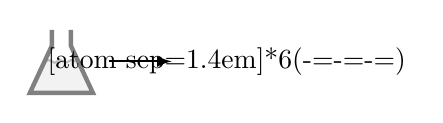
\begin{tikzpicture}
            \begin{scope}[xshift=-1cm,scale=0.4]
                \fill [gray!10] (-0.5,0) -- (-1,-1) -- (1,-1) -- (0.5,0);
                \draw [gray!50,thick,decorate,decoration={snake,segment length=4pt,amplitude=0.5pt}] (-0.5,0) -- (0.5,0);
    
                \draw [gray,ultra thick] (-0.3,1) -- (-0.3,0.5) -- (-1,-1) -- (1,-1) -- (0.3,0.5) -- (0.3,1);
            \end{scope}
            \draw [thick,-latex] (-0.4,0) -- (0.4,0);
            \node at (1.1,0) {\chemfig[atom sep=1.4em]{*6(-=-=-=)}};
        \end{tikzpicture}
        \caption{Why we study structure determination.}
        \label{fig:structureDeterminationRationale}
    \end{figure}
    \begin{itemize}
        \item With the naked eye, organic chemists see a flask with a colorless liquid. But we draw the skeletal diagram for benzene (which is a colorless liquid). What tools enable us to convert from the flask to the structure?
        \item Here's another reason: Suppose we run a brand new chemical reaction. Organic chemists do this all the time in research! How do we now what the product is? How do we know which atoms it contains, and in what arrangement?
    \end{itemize}
    \item Structure determination workflow.
    \begin{enumerate}
        \item Identify the atoms present.
        \begin{itemize}
            \item Questions to answer: What is the molecular formula?
            \item Relevant tools: Elemental analysis (EA) and mass spectrometry ("mass spec" or MS).
        \end{itemize}
        \item Identify the functional groups and substructures present.
        \begin{itemize}
            \item Questions to answer: Do we have ketones? Esters? Alcohols? Rings?
            \item Relevant tools: MS, infrared spectroscopy (IR), and nuclear magnetic resonance (NMR).\footnote{NMR is an organic chemist's best friend!}
        \end{itemize}
        \item Identify how all the functional groups fit together.
        \begin{itemize}
            \item Questions to answer: Are they close? Far apart? Ortho/meta/para? What stereochemistry?
            \item Relevant tools: NMR and X-ray diffraction.
        \end{itemize}
    \end{enumerate}
    \item We now begin talking about EA.
    \begin{itemize}
        \item History: Began development in the 1820s.
        \item Purpose: Determine which elements are present, and in what quantities (in a given sample).
    \end{itemize}
    \item In this course, we will apply EA to compounds containing carbon, hydrogen, and oxygen \emph{exclusively}.
    \begin{itemize}
        \item To reiterate, in an EA problem for this course, we will \emph{not} have to worry about any other elements.
        \item The typical EA technique for such compounds is \textbf{combustion analysis}.
    \end{itemize}
    \item \textbf{Combustion analysis}: Burn the sample and measure the products.
    \begin{itemize}
        \item All \ce{C} in the sample becomes \ce{CO2}.
        \item All \ce{H} in the sample becomes \ce{H2O}.
        \item \ce{O} is then determined via process of elimination, explained as follows.
    \end{itemize}
    \item Advanced techniques (beyond the scope of this class): Nitrogen to \ce{NO} or \ce{NO2}, sulfur to \ce{SO2}, etc.
    \item A schematic of combustion analysis.
    \begin{figure}[h!]
        \centering
        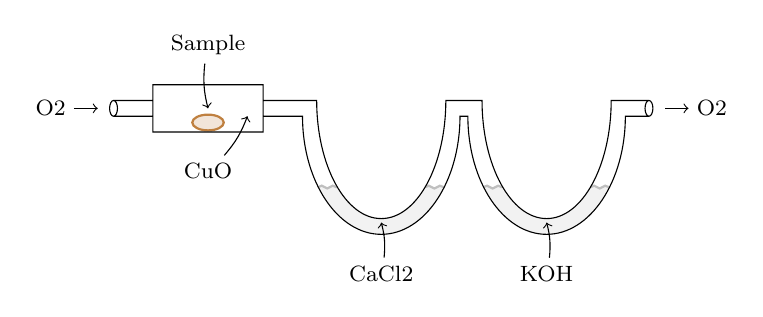
\begin{tikzpicture}
            \footnotesize
            \filldraw [draw=brown,thick,fill=brown!20] (0,-0.18) ellipse (2mm and 1mm);
            \node at (0,0.8) {Sample}
                edge[bend right=10,->] (0,0)
            ;
            \node at (0,-0.8) {\ce{CuO}}
                edge[bend right=10,->] (0.5,-0.1)
            ;
    
            \fill [gray!10] (1.4,-1)
                -- ({1.4+0.24},-1)
                arc[start angle=-140,end angle=-40,x radius=0.73cm,y radius=1.12cm]
                -- ({1.4+1.6},-1)
                arc[start angle=-40,end angle=-140,x radius=1.04cm,y radius=1.66cm]
                -- cycle
            ;
            \draw [gray!50,thick,decorate,decoration={snake,segment length=4pt,amplitude=0.5pt}] (1.4,-1) -- (1.64,-1);
            \draw [gray!50,thick,decorate,decoration={snake,segment length=4pt,amplitude=0.5pt}] (2.76,-1) -- (3,-1);
            \node at (2.2,-2.1) {\ce{CaCl2}}
                edge[bend right=10,->] (2.2,-1.45)
            ;
            \fill [gray!10] (3.5,-1)
                -- ({3.5+0.24},-1)
                arc[start angle=-140,end angle=-40,x radius=0.73cm,y radius=1.12cm]
                -- ({3.5+1.6},-1)
                arc[start angle=-40,end angle=-140,x radius=1.04cm,y radius=1.66cm]
                -- cycle
            ;
            \draw [gray!50,thick,decorate,decoration={snake,segment length=4pt,amplitude=0.5pt}] (3.5,-1) -- ({3.5+0.24},-1);
            \draw [gray!50,thick,decorate,decoration={snake,segment length=4pt,amplitude=0.5pt}] ({3.5+1.6-0.24},-1) -- ({3.5+1.6},-1);
            \node at (4.3,-2.1) {\ce{KOH}}
                edge[bend right=10,->] (4.3,-1.45)
            ;
    
            \draw
                (-1.2,0) ellipse (0.5mm and 1mm)
                (-1.2,0.1)  -- (-0.7,0.1)
                (-1.2,-0.1) -- (-0.7,-0.1)
                (-0.7,-0.3) rectangle (0.7,0.3)
                (0.7,-0.1) -- (1.2,-0.1)
                    arc[start angle=-180,end angle=0,x radius=1cm,y radius=1.5cm]
                    -- ++(0.1,0)
                    arc[start angle=-180,end angle=0,x radius=1cm,y radius=1.5cm]
                    -- ++(0.3,0)
                (0.7,0.1) -- (1.38,0.1)
                    arc[start angle=-180,end angle=0,x radius=0.82cm,y radius=1.5cm]
                    -- ++(0.46,0)
                    arc[start angle=-180,end angle=0,x radius=0.82cm,y radius=1.5cm]
                    -- ++(0.48,0)
                (5.6,0) ellipse (0.5mm and 1mm)
            ;
            \node at (-2,0) {\ce{O2}}
                edge [->] (-1.4,0)
            ;
            \node at (6.4,0) {\ce{O2}}
                edge [<-] (5.8,0)
            ;
        \end{tikzpicture}
        \caption{Combustion analysis schematic.}
        \label{fig:combustionAnalysis}
    \end{figure}
    \begin{itemize}
        \item Burn the sample in the presence of an oxidant such as cupric oxide (\ce{CuO}).
        \item Flow \ce{O2} into the combustion chamber to facilitate burning as well.
        \item The combusted gas then flows through a series of reaction containers.
        \begin{itemize}
            \item The first one contains a desiccant (like \ce{CaCl2}) that absorbs the water.
            \item The second one contains a base (like \ce{KOH}) that absorbs the \ce{CO2}.
        \end{itemize}
        \item The remaining oxygen flows out the end.
    \end{itemize}
    \item The \emph{analysis} part of combustion analysis.
    \begin{itemize}
        \item The amount of \ce{H} is equal to the change in mass of the \ce{CaCl2}.
        \begin{equation*}
            \Delta\text{mass}(\ce{CaCl2}) = \text{mass}(\ce{H2O})
            \to \text{ratio}(\ce{H})
        \end{equation*}
        \item The amount of \ce{C} is equal to the change in mass of the \ce{KOH}.
        \begin{equation*}
            \Delta\text{mass}(\ce{KOH}) = \text{mass}(\ce{CO2})
            \to \text{ratio}(\ce{C})
        \end{equation*}
        \item The amount of \ce{O} is equal to the change in mass of the sample.
        \begin{equation*}
            \text{mass}(\text{sample})-\text{mass}(\ce{H})-\text{mass}(\ce{C}) = \text{mass}(\ce{O})
             \to \text{ratio}(\ce{O})
        \end{equation*}
        \item Result: We get an \textbf{empirical formula} of the form \ce{C_{$x$}H_{$y$}O_{$z$}}. Remember that this is \emph{not} (necessarily) the \textbf{molecular formula}; it is \emph{only} a ratio of elements.
    \end{itemize}
    \item EA example: Let's burn \SI{0.5}{\gram} of propanol (\ce{C3H8O}).
    \begin{itemize}
        \item Suppose we obtain \SI{0.600}{\gram} \ce{H2O} and \SI{1.09}{\gram} \ce{CO2}.
        \item This means that there was \SI{0.067}{\gram} (\ce{H}) and \SI{0.300}{\gram} (\ce{C}) in the sample. The remaining \SI{0.133}{\gram} must then be due to \ce{O}.
        \item Therefore, the elements exist in a 3:8:1 (C:H:O) ratio.
        \item Bonus: Convert the masses to a ratio via stoichiometry.
        \begin{itemize}
            \item $
                \SI{0.600}{\gram}\ \ce{H2O}
                \times\dfrac{\SI{1}{\mole}\ \ce{H2O}}{\SI{18.02}{\gram}\ \ce{H2O}}
                \times\dfrac{\SI{2}{\mole}\ \ce{H}}{\SI{1}{\mole}\ \ce{H2O}}
                \times\dfrac{\SI{1.01}{\gram}\ \ce{H}}{\SI{1}{\mole}\ \ce{H}}
                = \SI{0.067}{\gram}\ (\ce{H})
            $
            \item $
                \SI{1.09}{\gram}\ \ce{CO2}
                \times\dfrac{\SI{1}{\mole}\ \ce{CO2}}{\SI{44.01}{\gram}\ \ce{CO2}}
                \times\dfrac{\SI{1}{\mole}\ \ce{C}}{\SI{1}{\mole}\ \ce{CO2}}
                \times\dfrac{\SI{12.01}{\gram}\ \ce{C}}{\SI{1}{\mole}\ \ce{C}}
                = \SI{0.300}{\gram}\ (\ce{C})
            $
            \item $
                \SI{0.5}{\gram}\ \text{propanol}
                -\SI{0.067}{\gram}\ (\ce{H})
                -\SI{0.300}{\gram}\ (\ce{C})
                = \SI{0.133}{\gram}\ (\ce{O})
            $
        \end{itemize}
    \end{itemize}
    \item A note on the previous example.
    \begin{table}[h!]
        \centering
        \small
        \renewcommand{\arraystretch}{1.4}
        \begin{tabular}{l|cc|ccc}
            \textbf{Name} & Propanol & Methyl ethyl ether & Formaldehyde & Acetic acid & Glucose\\
            \textbf{Structure} &
                \footnotesize\chemfig[atom sep=1em]{-[:30]-[:-30]-[:30]OH} &
                \footnotesize\chemfig[atom sep=1em]{-[:30]-[:-30]O-[:30]} &
                \footnotesize\chemfig[atom sep=1em,baseline=0.8em]{H-[:30](=[2]O)-[:-30]H} &
                \footnotesize\chemfig[atom sep=1em,baseline=0.8em]{-[:30](=[2]O)-[:-30]OH} &
                \footnotesize\chemfig[atom sep=1em]{?(-[:190]HO)-[:-50,1.4](-[:170]HO)-[:10,1.5](-[:-55]OH)-[:-10,1.5](-[:10]OH)-[:130]O-[:190]?(-[:150,0.7]-[2]OH)}\\
            \textbf{Emp. formula} & \ce{C3H8O} & \ce{C3H8O} & \ce{CH2O} & \ce{CH2O} & \ce{CH2O}\\
            \textbf{Mol. formula} & \ce{C3H8O} & \ce{C3H8O} & \ce{CH2O} & \ce{C2H4O2} & \ce{C6H12O6}\\
        \end{tabular}
        \caption{Questions that EA can't answer.}
        \label{tab:EAmols}
    \end{table}
    \begin{itemize}
        \item EA has given us the empirical formula, but it has \emph{not} confirmed that the sample is propanol. For example, methyl ethyl ether has the same empirical formula!
        \item Additionally, we don't yet have the molecular formula. Consider, for instance, the breadth of compounds with empirical formula \ce{CH2O}!
        \item Takeaway: EA gives you the empirical formula; we need MS to get the molecular formula (we'll see this on Friday), and we may need even more to get the atomic connectivity.
    \end{itemize}
    \item Application of EA to real-world chemistry.
    \begin{itemize}
        \item A home furnace burns natural gas --- which is mostly methane (\ce{CH4}) --- for heat.
        \item \textbf{Ideal combustion}\footnote{You can learn more about in a chemical engineering/ChemE course.} corresponds to the reaction
        \begin{equation*}
            \ce{CH4 + O2 -> CO2 + H2O}
        \end{equation*}
        \item Real-world combustion is incomplete; you make
        \begin{equation*}
            \ce{CH4 + air -> CO2 + H2O + NO2 + CO}
        \end{equation*}
        \item When a technician comes to your home, they analyze the flue gas (i.e., your furnace exhaust).
        \begin{itemize}
            \item Their analysis could determine that our combustion has too much \ce{O2}, which is called "air rich." This is inefficient and doesn't yield enough heat.
            \item They could also determine that you have too much \ce{CO2} and \ce{CO}, which is called "fuel rich." This yields too much soot and \ce{CO}. \ce{CO} can be dangerous and lead to carbon monoxide poisoning, which makes you sleepy before it kills you.
        \end{itemize}
        \item To measure this flue gas, though, they have a little handheld elemental analysis device!
    \end{itemize}
    \item Note that there is a relation between ideal/real-world combustion and the \ce{CuO} oxidant in Figure \ref{fig:combustionAnalysis}: The \ce{CuO} ensures that when we combust our EA sample, all the carbon is fully oxidized to \ce{CO2}! Without it, some \ce{CO} would be formed, and our stoichiometry would be thrown off.
\end{itemize}



\section{Mass Spectrometry}
\begin{itemize}
    \item \marginnote{9/6:}Lecture 1 recap.
    \begin{itemize}
        \item Elemental analysis (EA).
        \begin{equation*}
            \ce{SM + O2 ->[$\Delta$] CO2 + H2O}
        \end{equation*}
        \begin{itemize}
            \item SM means "\underline{s}tarting \underline{m}aterial."
            \item SM's we will focus on: Compounds of the form \ce{C_{$x$}H_{$y$}O_{$z$}}.
        \end{itemize}
        \item Empirical formula vs. molecular formula (see Table \ref{tab:EAmols}).
    \end{itemize}
    \item Today: Mass spectrometry (MS).
    \begin{itemize}
        \item Purpose: Convert empirical formulas to molecular formulas (and more!).
        \item Reading: \textcite{bib:Clayden}, Chapter 3.
    \end{itemize}
    \item Lecture outline.
    \begin{itemize}
        \item Mass spectrometer schematic.
        \item Mass spectrum elements.
        \item Fragmentation, and common types.
        \item Isotope effects in MS.
        \item Ionization methods.
    \end{itemize}
    \item \textbf{Mass spectrometry}: A structure determination technique that tells us the exact mass of molecules and their "fragments." \emph{Also known as} \textbf{MS}, "\textbf{mass spec}."
    \item Overview.
    \begin{center}
        \schemestart
        \chemfig{\cnc{M}}
        \arrow{-U>[\footnotesize$\textup{e}^-$][\footnotesize$2\textup{e}^-$]}
        \chemfig{\charge{20=\scriptsize +,-3=$\cdot$}{\cnc{M}}}
        \arrow(M--b)
        \subscheme{
            \chemfig{\charge{12=\scriptsize +}{\cnc{M$-b$}}}
            \+{3mm}
            \chemfig{\charge{[extra sep=1pt]30=$\cdot$}{\cnc{$b$}}}
        }
        \arrow(--a){0}[90,0.1]
        \subscheme{
            \chemfig{\charge{12=\scriptsize +}{\cnc{M$-a$}}}
            \+{3mm}
            \chemfig{\charge{[extra sep=1pt]30=$\cdot$}{\cnc{$a$}}}
        }
        \arrow(@b--c){0}[-90,0.1]
        \subscheme{
            \chemfig{\charge{12=\scriptsize +}{\cnc{M$-c$}}}
            \+{3mm}
            \chemfig{\charge{[extra sep=1pt]30=$\cdot$}{\cnc{$c$}}}
        }
        \arrow(@M--@a.west)
        \arrow(@M--@c.west)
        \schemestop
    \end{center}
    \begin{itemize}
        \item You have a sample --- denoted by $\cnc{M}$ --- that you bombard with electrons ($\e[-]$). When an electron hits a molecule of your sample, it knocks off one of the molecule's electrons (and flies off itself). This ionizes your molecule to a \textbf{radical cation}, denoted by $\cnc{M}\rc$ and called the \textbf{molecular ion}.
        \item This radical cation is unstable and fragments into a proper cation and a proper radical. The radical is usually not detected, but any cationic fragment produced --- the $\cnc{M$-a$}^+$, $\cnc{M$-b$}^+$, and $\cnc{M$-c$}^+$ above --- usually \emph{is} detected.
    \end{itemize}
    \item A (stepwise) schematic of a mass spectrometer.
    \begin{figure}[h!]
        \centering
        \footnotesize
        \begin{tikzpicture}
            \fill [gray!70,rotate around={-10:(2.3,0)}] (1.8,-0.8)
                -- node[below=1mm,black,digit]{5} (2.8,-0.8)
                -- (2.8,0.6)
                -- (1.8,0.6)
            ;
            \fill [white] (-0.3,0.1)
                -- (0,0.1)
                -- (0,0.5)
                -- (1.5,0.5)
                arc[start angle=90,end angle=35,radius=4cm]
                -- ++(-145:1)
                arc[start angle=35,end angle=90,radius=3cm]
                -- (0,-0.5)
                -- (0,-0.1)
                --(-0.3,-0.1)
            ;
    
            \draw [decorate,decoration={coil,segment length=2.2pt},rotate around={180:(0.4,0.4)}] (0.1,0.4) -- node[above=2mm,digit]{2} (0.7,0.4);
    
            \draw (0.2,-0.5)
                -- (0.2,-0.9)
                -- node[below=1mm,digit]{3} (0.5,-0.9)
                -- (0.5,-0.5)
            ;
            \draw [-stealth] (0.35,-0.45) -- ++(0,0.23);
            \draw [-stealth] (0.42,-0.45) -- ++(0.12,0.16);
            \draw [-stealth] (0.28,-0.45) -- ++(-0.12,0.16);
    
            \draw
                (-0.3,0) ellipse (0.3mm and 1mm)
                (-0.3,0.1) -- (0,0.1)
                    -- (0,0.5)
                    -- (1.5,0.5)
                    arc[start angle=90,end angle=35,radius=4cm] coordinate (b) node[right=1mm,digit]{6}
                (-0.3,-0.1) -- (0,-0.1)
                    -- (0,-0.5)
                    -- (1.5,-0.5)
                    arc[start angle=90,end angle=35,radius=3cm] coordinate (a) %node[left=2mm,digit]{6}
            ;
            \draw
                (1,0.5) arc[start angle=90,end angle=-90,x radius=1mm,y radius=5mm]
                (1.3,0.5) arc[start angle=90,end angle=-90,x radius=1mm,y radius=5mm]
                (0.9,0.02)  -- ++(0.2,0)
                (0.9,-0.02) -- ++(0.2,0)
                (1.2,0.02)  -- ++(0.2,0)
                (1.2,-0.02) -- ++(0.2,0)
            ;
            \draw
                (1,0.5) arc[start angle=90,end angle=270,x radius=1mm,y radius=5mm]
                (1.3,0.5) arc[start angle=90,end angle=270,x radius=1mm,y radius=5mm]
            ;
            \node [below,digit] at (1.15,-0.6) {4};
            \draw [rotate=-55] ($(a)!0.5!(b)+(0,0.5)$) arc[start angle=90,end angle=-90,x radius=1mm,y radius=5mm];
            \draw [rotate=-55] ($(a)!0.5!(b)+(0,0.5)$) arc[start angle=90,end angle=270,x radius=1mm,y radius=5mm];
    
            \node [label={[above,digit]1}] at (-1.8,0) {Sample}
                edge [dashed,->] (-0.45,0)
            ;
            \draw [dashed,->] (-0.1,0) -- (0.85,0);
            \draw [dashed,->] (1.45,0)
                -- (1.5,0)
                arc[start angle=90,end angle=49,radius=1.9cm] %node[circle,fill,inner sep=1pt]{}
                -- ++({49-90}:1.65)
            ;
            \draw [dashed,->] (1.45,0)
                -- (1.5,0)
                arc[start angle=90,end angle=57,radius=2.3cm] %node[circle,fill,inner sep=1pt]{}
                -- ++({57-90}:1.8)
            ;
            \draw [dashed,->] (1.45,0)
                -- (1.5,0)
                arc[start angle=90,end angle=63,radius=2.8cm] %node[circle,fill,inner sep=1pt]{}
                -- ++({63-90}:1.93)
            ;
        \end{tikzpicture}
        \caption{Mass spectrometer schematic.}
        \label{fig:MSschematic}
    \end{figure}
    \begin{enumerate}
        \item The sample is injected into a curved tube.
        \item A heater vaporizes the sample.
        \item An electron source (also known as an electron gun) shoots electrons at the vaporized sample, ionizing it. The ionized sample starts fragmenting.
        \item The fragments encounter a series of negatively charged plates with slits in the middle. These negatively charged plates accelerate the positively charged cations.
        \item A magnet deflects the accelerated, positively charged ions. The magnet deflects them based on their \textbf{mass-to-charge ratio}. Because of physics, the lightest ions are deflected the most, and the heaviest ions are deflected the least.
        \item A detector records where the ions hit. This data is converted into a mass-to-charge ratio for each ion. This yields a spectrum of all the fragments' masses.
    \end{enumerate}
    \item \textbf{Mass-to-charge ratio} (of a cation): The cation's mass divided by its net charge. \emph{Denoted by} $\bm{m/z}$.
    \begin{itemize}
        \item For the purposes of this class, $z=1$.
    \end{itemize}
    \item Example mass spectrum: Acetone (\,{\tiny\chemfig[baseline=1mm,atom sep=1em,bond offset=1pt,fixed length=false]{-[:30](=[2]O)-[:-30]}}\,).
    \begin{figure}[H]
        \centering
        \begin{tikzpicture}[xscale=0.16,yscale=0.04]
            \small
            \node [rotate=90] at (-5.875,50) {Relative Intensity};
            \node [below=5mm] at (35,0) {$m/z$};
    
            \footnotesize
            \draw (-0.625,100) node[left]{$100$} -- ++(1.125,0);
            \foreach \x in {10,20,...,60} {
                \draw (\x,2.5) -- ++(0,-5) node[below]{$\x$};
            }
    
            \draw [orange,ultra thick]
                (15,0) -- ++(0,14) node[above=1mm,black,thin,digit]{15} node[above=6mm,black]{$\cnc{M$-43$}^+=\cnc{CH3}^+$}
                (27,0) -- ++(0,1)
                (28,0) -- ++(0,1)
                (29,0) -- ++(0,1)
                (43,0) -- ++(0,100) node[above=1mm,black,thin,digit]{43} node[above=6mm,black]{${}^{\color{white}+}\cnc{M$-15$}^+=[\chemfig[atom sep=1.4em,fixed length=false,bond sep=2pt]{H_3C-~O}]^+$}
                (44,0) -- ++(0,3)
                (58,0) -- ++(0,26) node[above=1mm,black,thin,digit]{58} node[above=6mm,black]{${}^{\color{white}+}\cnc{M}^+=\Big[{\tiny\chemfig[baseline=1.3mm,atom sep=1em,bond offset=1pt,fixed length=false]{-[:30](=[2]O)-[:-30]}}\Big]^+$}
                (59,0) -- ++(0,2)
            ;

            \draw (0,110) -- (0,0) -- (70,0);
        \end{tikzpicture}
        \vspace{-0.5em}
        \caption{Mass spectrum of acetone.}
        \label{fig:MSacetone}
    \end{figure}
    \begin{itemize}
        \item The $x$-axis is the mass-to-charge ratio, and the $y$-axis is the "relative intensity" of each peak.
        \begin{itemize}
            \item If a certain fragment gets produced more than another (and hence recorded more than it), we say it has a "higher relative intensity."
        \end{itemize}
        \item We identify two special types of peaks in a mass spectrum: The \textbf{parent peak} and the \textbf{base peak}. In the case of acetone\dots
        \begin{itemize}
            \item The parent peak lies at 58;
            \item The base peak lies at 43.
        \end{itemize}
        \item The peak at 15 also has a relatively large magnitude, and from the fact that the mass of a methyl cation is approximately 15, we can infer that this peak corresponds to the methyl cation fragment.
        \begin{itemize}
            \item Notice that its intensity is significantly lower than the intensity of the base peak because we may recall from Orgo I that the methyl cation is a far less stable cation than the resonance-stabilized, secondary acylium ion at 43.
        \end{itemize}
        \item There are a number of smaller peaks, too, but they give less information.
        \item Note that the major peaks may be appropriately referred to by \emph{any} of the three nomenclature methods in Figure \ref{fig:MSacetone}: By exact mass, by $\cnc{M$-a$}^+$, and/or by structure.
    \end{itemize}
    \item \textbf{Parent peak}: The peak in a mass spectrum corresponding to the molecular ion.
    \begin{itemize}
        \item The parent peak is always the rightmost peak in the spectrum.\footnote{Excepting isotope effects; discussed later in this lecture.} This is because it is created by the heaviest ion, and you can't have more mass than your initial molecule!
        \item It is typically \emph{not} the tallest peak in the spectrum.
        \item Useful information: It gives the molecular weight of the molecule.
    \end{itemize}
    \item \textbf{Base peak}: The tallest peak in a mass spectrum.
    \begin{itemize}
        \item The base peak corresponds to the fragment that the molecule forms most preferentially, which is usually also the most stable fragment.
    \end{itemize}
    \item \textbf{Fragmentation peak}: Any peak to the left of the parent peak.
    \item Maxim: Molecules fragment in predictable ways to form stable cations.
    \item At this point, let's formally define \textbf{fragmentation}.
    \item \textbf{Fragmentation}: The formation of stable(-ish) cations.
    \begin{itemize}
        \item Recall from Orgo I (review your notes on cation stability!!) that stable cations tend to be more substituted, delocalized, atom-stabilized (e.g., close to a heteroatom), etc. 
    \end{itemize}
    \item Let's now discuss some common species that we analyze via MS --- and how they fragment.
    \item Alkane fragmentation: Preferentially break bonds to get more substituted (e.g., $2^\circ$ \& $3^\circ$) carbocations.
    \item Example: 2-methylbutane (\,{\tiny\chemfig[baseline=0.7mm,atom sep=1em,bond offset=1pt,fixed length=false]{-[:30](-[2])-[:-30]-[:30]}}\,).
    \begin{figure}[H]
        \centering
        \footnotesize
        \setchemfig{atom sep=1.4em}
        \schemestart
            \chemfig{-[:30](-[@{1}2])-[@{2}:-30]-[:30]}
            \arrow(--.174)
            \chemname{
                \chemleft[
                    \chemfig{-[:30](-[2])-[:-30]-[:30]}
                \chemright]
            }{$m/z=72$\\parent (minor)}
            \+{,,2mm}
            \chemname{
                \chemleft[
                    \chemfig{-[:30]\charge{[extra sep=5pt]90=$\oplus$}{}(-[2,,,,opacity=0])-[:-30]-[:30]}
                \chemright]
            }{$m/z=57$\\(major)}
            \+{,,2mm}
            \chemname{
                \chemleft[
                    \chemfig{-[:30]\charge{[extra sep=4pt]-30=$\oplus$}{}(-[2])-[:-30,,,,opacity=0]}
                \chemright]
            }{$m/z=43$\\(major)}
            \arrow{0}[,0.1]\+{,,2.5em}\arrow(--.165){0}[0,0.1]
            \chemname[1.2em]{
                \chemleft[
                    \chemfig{Et}
                \chemright]
            }{$m/z=29$\\(minor)}
            \arrow{0}[,0.1]\+{,,3.43em}\arrow{0}[0,0.1]
            \chemname[1.2em]{
                \chemleft[
                    \chemfig{Me}
                \chemright]
            }{$m/z=15$\\(minor)}
        \schemestop
        \hspace{-2mm}
        \chemmove{
            \draw [-,rex] ($(1)+(180:0.18)$) node[circle,draw,fill=white,inner sep=1pt]{} -- ($(1)+(0:0.18)$) node[circle,draw,fill=white,inner sep=1pt]{};
            \draw [-,rex] ($(2)+(-120:0.18)$) node[circle,draw,fill=white,inner sep=1pt]{} -- ($(2)+(60:0.18)$) node[circle,draw,fill=white,inner sep=1pt]{};
        }
        \begin{tikzpicture}[remember picture,overlay]
            % \draw (-13,0.37) -- ++(13,0);
            % \draw (-13,-0.19) -- ++(13,0);
            \node at (-8.82,0.65) {\tiny$\rc$};
            \node at (-1.96,0.38) {${}^+$};
            \node at (0,0.38) {${}^+$};
        \end{tikzpicture}
        \caption{Fragmentation of alkanes.}
        \label{fig:fragAlkane}
    \end{figure}
    \begin{itemize}
        \item All these peaks will appear, but the tallest will correspond to the species labeled "major" above.
    \end{itemize}
    \item Alcohol fragmentation.
    \begin{itemize}
        \item Dehydration: Yields an $\cnc{M$-18$}^+$ peak, corresponding to the loss of water.
        \item $\alpha$-cleavage: Leads to a resonance-stabilized product.
    \end{itemize}
    \item Example: Pentan-3-ol (\,{\tiny\chemfig[baseline=1mm,atom sep=1em,bond offset=1pt,fixed length=false]{(-[:150])-[:30](-[2]OH)-[:-30]-[:30]}}\,).
    \begin{figure}[h!]
        \centering
        \footnotesize
        \setchemfig{atom sep=1.4em}
        \begin{subfigure}[b]{0.49\linewidth}
            \centering
            \schemestart
                \chemname{
                    \chemfig{-[:-30]-[:30](-[@{1}2]OH)-[:-30]-[:30]}
                }{$m/z=88$}
                \arrow
                \chemname{
                    \chemfig{-[:-30]-[:30](-[2,,,,opacity=0]\phantom{OH})=_[:-30]-[:30]}
                }{$m/z=70$}
            \schemestop
            \chemmove{
                \draw [-,rex] ($(1)+(180:0.18)$) node[circle,draw,fill=white,inner sep=1pt]{} -- ($(1)+(0:0.18)$) node[circle,draw,fill=white,inner sep=1pt]{};
            }
            \caption{Dehydration.}
            \label{fig:fragOHa}
        \end{subfigure}
        \begin{subfigure}[b]{0.49\linewidth}
            \centering
            \schemestart
                \chemname{
                    \chemfig{-[:-30]-[:30](-[2]OH)-[@{2}:-30]-[:30]}
                }{$m/z=88$}
                \arrow
                \chemname{
                    \chemleft[\subscheme{
                        \chemfig{-[:-30]-[:30]\charge{[extra sep=4pt]-30=$\oplus$}{}-[2]OH}
                        \arrow{<->}
                        \chemfig{-[:-30]-[:30]=^[2]\charge{[extra sep=4pt]180=$\oplus$}{O}H}
                    }\chemright]
                }{$m/z=59$}
            \schemestop
            \chemmove{
                \draw [-,rex] ($(2)+(-120:0.18)$) node[circle,draw,fill=white,inner sep=1pt]{} -- ($(2)+(60:0.18)$) node[circle,draw,fill=white,inner sep=1pt]{};
            }
            \caption{$\alpha$-cleavage.}
            \label{fig:fragOHb}
        \end{subfigure}
        \caption{Fragmentation of alcohols.}
        \label{fig:fragOH}
    \end{figure}
    \item Ketone fragmentation.
    \begin{itemize}
        \item $\alpha$-cleavage: Leads to a resonance-stabilized product, once again.
        \item McLafferty rearrangement: Only happens for ketones with a $\gamma$-proton.
        \begin{itemize}
            \item We select for this type of ketone because in this case, we can form a six-membered transition state. Recall that six-membered transition states are super stable in organic chemistry!
            \item This fragmentation leads to a charged enol (that we see in the spectrum) and an uncharged olefin (that we don't see in the spectrum).
        \end{itemize}
    \end{itemize}
    \item Example: Hexanones.
    \begin{figure}[h!]
        \centering
        \footnotesize
        \setchemfig{atom sep=1.4em}
        \begin{subfigure}[b]{\linewidth}
            \centering
            \schemestart
                \chemname{
                    \chemfig{(-[:-150])-[:-30]-[@{3}:30](=[2]O)-[@{2}:-30]-[:30]}
                }{$m/z=100$}
                \arrow(.11--.174)
                \chemname{
                    \chemleft[
                        \chemfig{(-[:-150])-[:-30]-[:30]~[:30]\charge{[extra sep=5pt]100=$\oplus$}{O}}
                    \chemright]
                }{$m/z=71$}
                \+
                \chemname{
                    \chemleft[
                        \chemfig{(~[:150]\charge{[extra sep=5pt]80=$\oplus$}{O})-[:-30]-[:30]}
                    \chemright]
                }{$m/z=57$}
            \schemestop
            \chemmove{
                \draw [-,rex] ($(2)+(-120:0.18)$) node[circle,draw,fill=white,inner sep=1pt]{} -- ($(2)+(60:0.18)$) node[circle,draw,fill=white,inner sep=1pt]{};
                \draw [-,rex] ($(3)+(-60:0.18)$) node[circle,draw,fill=white,inner sep=1pt]{} -- ($(3)+(120:0.18)$) node[circle,draw,fill=white,inner sep=1pt]{};
            }
            % \begin{tikzpicture}[remember picture,overlay]
            %     \draw (-5,0.88) -- ++(13,0);
            %     \draw (-5,0.32) -- ++(13,0);
            % \end{tikzpicture}
            \caption{$\alpha$-cleavage.}
            \label{fig:fragKetonea}
        \end{subfigure}\\[2em]
        \begin{subfigure}[b]{\linewidth}
            \centering
            \schemestart
                \chemfig{-[:30](=[2]O)-[:-30]\charge{[extra sep=4pt]-90=$\alpha$}{}-[:30]\charge{[extra sep=4pt]90=$\beta$}{}-[:-30]\charge{[extra sep=4pt]-90=$\gamma$}{}-[:30]}
                \arrow(--.170)
                \chemname[0em]{
                    \chemleft[
                        \chemfig[atom sep=2.5em,fixed length=false]{-[:30](=[@{db}2]O)-[@{sb2}:-30]-[@{sb3}:30]-[@{sb4}2](-[@{sb5}:150]H-[@{sb6,0.3}:-150,,,,opacity=0])-[:30]}
                    \chemright]
                }{$m/z=100$}
                \arrow(.10--.151)
                \chemname[1.5em]{
                    \chemleft[
                        \chemfig{-[:30](-[2]OH)=_[:-30]}
                    \chemright]
                }{$m/z=58$}
                \arrow(--.210){0}[,0]\+{,,3.9mm}
                \chemfig{=_[2]-[:30]}
            \schemestop
            \chemmove{
                \draw [curved arrow={2pt}{1pt},arrows={-Stealth[harpoon,flex]}] (db) to[out=10,in=-70,out looseness=2,in looseness=1] (sb6);
                \draw [curved arrow={2pt}{1pt},arrows={-Stealth[harpoon,flex,swap]}] (db) to[out=-10,in=70,out looseness=2,in looseness=1.5] (sb2);
                \draw [curved arrow={1pt}{1pt},arrows={-Stealth[harpoon,flex]}] (sb3) to[out=130,in=50,out looseness=2,in looseness=1.5] (sb2);
                \draw [curved arrow={1pt}{1pt},arrows={-Stealth[harpoon,flex,swap]}] (sb3) to[out=110,in=-170,out looseness=2,in looseness=1.5] (sb4);
                \draw [curved arrow={1pt}{1pt},arrows={-Stealth[harpoon,flex]}] (sb5) to[out=-110,in=170,out looseness=2,in looseness=1.5] (sb4);
                \draw [curved arrow={1pt}{1pt},arrows={-Stealth[harpoon,flex,swap]}] (sb5) to[out=-130,in=-50,out looseness=2,in looseness=1] (sb6);
            }
            \begin{tikzpicture}[remember picture,overlay]
                % \draw (-5,1.45) -- ++(13,0);
                % \draw (-5,0.32) -- ++(13,0);
                \node at (-4.24,1.08) {\tiny$\rc$};
                \node at (-1.12,0.8) {\tiny$\rc$};
            \end{tikzpicture}
            \caption{McLafferty rearrangement.}
            \label{fig:fragKetoneb}
        \end{subfigure}
        \caption{Fragmentation of ketones.}
        \label{fig:fragKetone}
    \end{figure}
    \item Isotope effects.
    \item Principle: Mass spectrometry weighs individual molecules, so molecules containing a heavier (or lighter) isotope will appear separate from other molecules in the mass spectrum.
    \item Atoms with notable isotope effects.
    \begin{figure}[H]
        \centering
        \begin{subfigure}[b]{0.17\linewidth}
            \centering
            \begin{tikzpicture}
                \draw [orange,ultra thick]
                    (0.8,0) -- ++(0,1.2)
                    (0.96,0) -- ++(0,0.05)
                ;

                \draw (0,1.4) -- (0,0) -- (1.8,0);
            \end{tikzpicture}
            \caption{Carbon.}
            \label{fig:isotopeEffectsMSa}
        \end{subfigure}
        \begin{subfigure}[b]{0.17\linewidth}
            \centering
            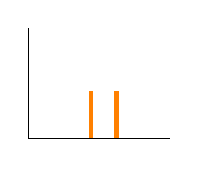
\begin{tikzpicture}
                \draw [orange,ultra thick]
                    (0.8,0) -- ++(0,0.6)
                    (1.12,0) -- ++(0,0.6)
                ;
                
                \draw (0,1.4) -- (0,0) -- (1.8,0);
            \end{tikzpicture}
            \caption{Bromine.}
            \label{fig:isotopeEffectsMSb}
        \end{subfigure}
        \begin{subfigure}[b]{0.17\linewidth}
            \centering
            \begin{tikzpicture}
                \draw [orange,ultra thick]
                    (0.8,0) -- ++(0,0.9)
                    (1.12,0) -- ++(0,0.3)
                ;
                
                \draw (0,1.4) -- (0,0) -- (1.8,0);
            \end{tikzpicture}
            \caption{Chlorine.}
            \label{fig:isotopeEffectsMSc}
        \end{subfigure}
        \caption{Isotope effects in MS.}
        \label{fig:isotopeEffectsMS}
    \end{figure}
    \begin{itemize}
        \item Carbon: The $\ce{{}^12C}:\ce{{}^13C}$ ratio is $99:1$.
        \begin{itemize}
            \item Implication: For every $\cnc{M}\rc$, we see 1\% $\cnc{M$+1$}\rc$.
            \item This is why we see tiny "shadow" peaks to the right of the parent peak and base peak in Figure \ref{fig:MSacetone}!
            \begin{itemize}
                \item Note that the "shadow" of the parent peak is 3\% its height (not 1\%) because there are \emph{three} carbons in the acetone molecular ion.
                \item Similarly, the "shadow" of the base peak is 2\% its height because there are \emph{two} carbons in the acylium ion.
            \end{itemize}
        \end{itemize}
        \item Bromine: The $\ce{{}^79Br}:\ce{{}^81Br}$ ratio is $1:1$.
        \begin{itemize}
            \item Implication: The $\cnc{M}\rc$ and $\cnc{M$+2$}\rc$ peaks exist in a $1:1$ ratio, i.e., have the same height/relative intensity.
            \item The splitting of the molecular ion peak into two such peaks is a super recognizable, distinct, and useful fingerprint of bromine-containing compounds!
        \end{itemize}
        \item Chlorine: The $\ce{{}^35Cl}:\ce{{}^37Cl}$ ratio is $3:1$.
        \begin{itemize}
            \item Implication: The $\cnc{M}\rc$ and $\cnc{M$+2$}\rc$ peaks exist in a $3:1$ ratio.
            \item Similar to bromine, this peak splitting is a fingerprint of chlorine-containing compounds.
        \end{itemize}
    \end{itemize}
    \item Combining everything we've learned up to this point, let's do another example.
    \item Example: Benzyl chloride (\,{\tiny\chemfig[baseline=0.5mm,atom sep=1em,bond offset=1pt,fixed length=false]{*6(=-=(--[:-30]Cl)-=-)}}\,).
    \begin{figure}[h!]
        \centering
        \begin{tikzpicture}[xscale=0.08,yscale=0.04]
            \small
            \node [rotate=90] at (-11.75,50) {Relative Intensity};
            \node [below=5mm] at (80,0) {$m/z$};
    
            \footnotesize
            \draw (-1.25,100) node[left]{$100$} -- ++(2.5,0);
            \foreach \x in {50,100,150} {
                \draw (\x,2.5) -- ++(0,-5) node[below]{$\x$};
            }
    
            \draw [orange,ultra thick]
                (40,0) -- ++(0,8) node[above=1mm,black,thin,digit]{40}
                (65,0) -- ++(0,12) node[above=1mm,black,thin,digit]{65}
                (91,0) -- ++(0,100) node[above=1mm,black,thin,digit,label={[right=2mm,yshift=-2mm,black]
                    \chemleft[
                        \chemfig[atom sep=1em]{*6(=-=(-\charge{[extra sep=5pt]90=$\oplus$}{})-=-)}
                    \chemright]
                }]{91}
                (92,0) -- ++(0,7) node[above right=1mm,black,thin,digit]{92}
                (126,0) -- ++(0,27) node[above=1mm,black,thin,digit,label={[right=2.5mm,yshift=2mm,black]
                    \chemleft[
                        \chemfig[atom sep=1em]{*6(=-=(--[:-30]{}^{36}Cl)-=-)}
                    \chemright{]^\rc}
                }]{126}
                (128,0) -- ++(0,9) node[above right=1mm,black,thin,digit,label={[right=2.5mm,yshift=-2mm,black]
                    \chemleft[
                        \chemfig[atom sep=1em]{*6(=-=(--[:-30]{}^{38}Cl)-=-)}
                    \chemright{]^\rc}
                }]{128}
            ;
    
            \draw (0,110) -- (0,0) -- (160,0);
        \end{tikzpicture}
        \vspace{-0.5em}
        \caption{Mass spectrum of benzyl chloride.}
        \label{fig:MSBnCl}
    \end{figure}
    \begin{itemize}
        \item The parent peak will lie at 126, and the corresponding chlorine isotope peak will lie at 128 and be one-third the height.
        \item The base peak will lie at 91, and the corresponding carbon isotope peak will lie at 92 and be 7\% the height (to account for the 7 carbons in the benzylic cation that may be heavy).
        \begin{itemize}
            \item It will correspond to the most stable fragment, which in this case is the benzylic cation.
            \item The benzylic cation is super stable because its positive charge can be resonance delocalized to four different atoms!
            \item A large peak at $m/z=91$ strongly suggests the presence of an aromatic system.
        \end{itemize}
        \item This example focused on predicting the peaks in a mass spectrum based on reasonable fragmentation patterns. But what if we are given the mass spectrum? What data can we pull out then?
    \end{itemize}
    \item To answer this question, here are some guidelines for the interpretation of mass spectra.
    \item Guidelines for interpretation.
    \begin{itemize}
        \item The parent peak provides the molecular weight of the molecule.
        \begin{itemize}
            \item This allows you to convert an empirical formula obtained from EA to the molecular formula.
        \end{itemize}
        \item The parent peak also reveals key atoms via distinct isotopic fingerprints.
        \begin{itemize}
            \item Examples include bromine and chlorine.
            \item An additional one is the \textbf{nitrogen rule}.
        \end{itemize}
        \item Fragmentation patterns can identify substructures.
        \begin{itemize}
            \item Recall from Lecture 1 (9/4) that identifying substructures is part of the second step of the structure determination workflow!
            \item Common fragments:
            \begin{itemize}
                \item Loss of a methyl group is $-15$.
                \item Loss of an OH group is $-17$.
                \item Loss of \ce{H2O} is $-18$.
                \item Loss of \ce{CO2} is $-44$.
                \item Loss of a \ce{{}^$t$Bu} group is $-57$.
            \end{itemize}
            \item Look at the $m/z$ of the fragments \emph{and} the difference in $m/z$ between certain fragments.
            \begin{itemize}
                \item Example: Maybe a certain fragment is formed by losing both a methyl group \emph{and} water.
            \end{itemize}
        \end{itemize}
        \item Important note: These guidelines are just a guide; we will need multiple forms of evidence to support an assignment.
    \end{itemize}
    \item \textbf{Nitrogen rule}: If you have an odd number of nitrogen in a molecule, you will get an odd molecular weight.
    \begin{itemize}
        \item The basis for this rule lies in the fact that nitrogen is trivalent but has an even mass.
        \begin{itemize}
            \item This means that nitrogen tends to bond an odd number of groups (specifically, 3), making the overall mass odd.
        \end{itemize}
        \item Examples: Ammonia has an odd mass of $17=14+1+1+1$ and methylamine has an odd mass of $31=(14+1+1)+(12+1+1+1)$, while methane has an even mass of $16=12+1+1+1+1$ and ethane has an even mass of $30=(12+1+1+1)+(12+1+1+1)$.
        \item You can read more about the nitrogen rule \href{https://en.wikipedia.org/wiki/Nitrogen_rule}{here}.
        \item Implication: If you see an odd molecular weight, you \emph{might} have a nitrogen present!
    \end{itemize}
    \item Types of ionization.
    \item \textbf{Electron ionization}: A beam of electrons. \emph{Denoted by} \textbf{EI}. \emph{Also known as} \textbf{hard ionization}.
    \begin{itemize}
        \item This is the method we are using in this class.
    \end{itemize}
    \item \textbf{Electrospray ionization}: Forms charged droplets. \emph{Denoted by} \textbf{ESI}. \emph{Also known as} \textbf{soft ionization}.
    \begin{itemize}
        \item ESI causes less fragmentation.
        \item One implication of this is that you observe a larger parent peak.
        \item Another consequence is that ESI can analyze a broader range of compounds via mass spectrometry than EI can, since some sensitive compounds (like proteins) would never survive an electron beam.
        \begin{itemize}
            \item Nobel Prize in Chemistry (2002) for this application of MS to biology!
        \end{itemize}
    \end{itemize}
    \item \textbf{High resolution mass spectrometry}. \emph{Denoted by} \textbf{HRMS}.
    \begin{itemize}
        \item In "normal" low-resolution mass spectrometry (LRMS), both \ce{N2} and \ce{C2H4} have $m/z=28$.
        \item In HRMS, \ce{N2} has $m/z=28.0061$ and \ce{C2H4} has $m/z=28.0314$.
    \end{itemize}
    \item HRMS leads nicely into our application for today!
    \item Application of MS to real-world chemistry: Isotopic signatures.
    \begin{itemize}
        \item Today, you learned that the $\ce{{}^12C}:\ce{{}^13C}$ ratio is $99:1$.
        \begin{itemize}
            \item In reality, this is an \emph{average} value.
            \item The actual ratio of isotopes is globally uneven, and we as humans have mapped it.
        \end{itemize}
        \item Indeed, isotope abundances vary by time and location due to air patterns, etc.
        \item For example, Montana is home to 2\% more \ce{{}^13C} than Florida!
        \item Implication: We can tell if a narcotic is made in the US (and where) or another country based on the isotopic abundance in it.
        \item We can also track where a person, drug, or uranium sample is from.
        \begin{itemize}
            \item Naturally, the government is very interested in this technology :)
        \end{itemize}
        \item You can also tell if a person eats corn or rice because this leads to different ratios of nitrogen isotopes in our bodies.
    \end{itemize}
\end{itemize}




\end{document}